\section{\secsumconj}
\label{sec_sum_conj}

Although we have a notation for sums and products, we still need to go through a process to evaluate a sum and product.  First, we need to calculate each term.  Next, we need to add or multiply.  In some cases, we can find an explicit formula for a sum or a product, which allows us to evaluate using a formula. In this section, we introduce partial sums and partial products and use them to conjecture explicit formulas.

%%%%%%%%%%%%%%%%%%%%%%%%%%%%%%%%%%%%%%%%%%

\newcommand{\subsumconj}{Sum Conjectures}
\subsection{\subsumconj}
\label{sub_sum_conj}

We start with sums.  

\begin{defn}[Partial sums]
\label{defn_partial_sum}
    Consider a list of numbers $a_s, a_{s+1}, a_{s+2}, \ldots, a_n$ for some integers $s$ and $n$. 
        \begin{apart}
            \item For the sum  
                $$\sum_{k=s}^n a_k =a_s + a_{s+1}+a_{s+2}+\ldots+a_n,$$
            the \vocab{partial sums} are 
                \begin{align*}
                    \sum_{k=s}^s a_k & =a_s, \\
                    \sum_{k=s}^{s+1} a_k & =a_s+a_{s+1}, \\
                    \sum_{k=s}^{s+2} a_k & =a_s+a_{s+1}+a_{s+2},
                \end{align*}
            and so on.  For example, for the sum   
                $$\sum_{k=1}^n 2 =2 + 2 + 2 + \ldots + 2,$$
            the partial sums are  
                \begin{align*}
                    \sum_{k=1}^1 2 &=2, \\
                    \sum_{k=1}^2 2 &=2+2=4,\\
                    \sum_{k=1}^3 2 &=2+2+2=6,
                \end{align*}
            and so on.
            \item The \vocab{sequence of partial sums} is 
                $$a_s, a_s+a_{s+1},a_s+a_{s+1}+a_{s+2}, \ldots.$$
            For example, the sequence of partial sums in our example begins $$2, 4, 6, \ldots.$$
        \end{apart}
\end{defn}

We focus on finite sums, but we mention, for readers who have studied calculus, that these are the same partial sums used to define infinite series. 

There is a shorthand notation for calculating partial sums that we introduce in our next example, where we revisit the sum from \Cref{defn_partial_sum}.

\begin{exam}[Conjecture explicit form of sum of constant]
\label{exam_partial_sums_conj_constant}
    Consider the sum $$\sum_{k=1}^n 2 =2 + 2 + 2 + \ldots + 2.$$  
        \begin{apart}
            \item Calculate the partial sums.
                \begin{soln}
                    We display the partial sums using a shorthand in \Cref{fig_part_sums_constant}.  At each $+$ sign, we draw a line and record the sum from the beginning to that line.
                \end{soln}
                \begin{figure}[hbtp]
                    \centering
                    \scalebox{0.75}{\input{Tikz/partial_sums_constant}}
                    \caption{Calculating partial sums for $\displaystyle \sum_{k=1}^n2$.}
                    \label{fig_part_sums_constant}
                \end{figure}
            \item Display the partial sums in a table.
                \begin{soln}
                    We are interested in finding an explicit formula sum as a function of $n$, so it is helpful to have the partial sums in a table, as shown in \Cref{tab_partial_sums_constant}.
                \end{soln}
                \begin{table}[hbtp]
                    \centering
                    \begin{tabular}{c|c|c|c|c|c|c}
                        $n$ & 1 & 2 & 3 & 4 & 5 & 6 \\ \hline
                        partial sum & 2 & 4 & 6 & 8 & 10 & 12 \\ \hline
                        pattern & 2(1) & 2(2) & 2(3) & 2(4) & 2(5) & 2(6)
                    \end{tabular}
                    \caption{Partial sums for $\displaystyle \sum_{k=1}^n2$.}
                    \label{tab_partial_sums_constant}
                \end{table}
            \item Use pattern recognition to conjecture an explicit form.
                \begin{soln}
                    We notice that each partial sum is twice the index $n$, and add another row to our table to show the pattern.  We conjecture $\displaystyle \sum_{k=1}^n2=2n$, which is no surprise since
                    $$ \sum_{k=1}^n2 = \underbrace{2 +2+ \ldots + 2}_{n \text{ times}}=2n.$$
                \end{soln}
        \end{apart}
\end{exam}

Observe that we can use each partial sum to calculate the next partial sum without having to add from the beginning.  For example, once we calculate $\displaystyle \sum_{k=1}^32 = 2+2+2 = 6$, we can calculate 
    $$\displaystyle \sum_{k=1}^42 = 2+2+2+2 = (2+2+2)+2=6+2=8.$$  
That is, the new partial sum is equal to the previous partial sum plus the new term.
We state this result in general.

\begin{rem}[Recursive definition of partial sums]
\label{rem_rec_def_partial_sum} 
    Consider a list of numbers $a_s, a_{s+1}, a_{s+2}, \ldots, a_n$ for some integers $s$ and $n$. Then
        \begin{align*}
            \sum_{k=s}^n a_k & = a_s + a_{s+1} + \ldots + a_{n-1} + a_n \\
            & = (a_s + a_{s+1} + \ldots + a_{n-1}) + a_n \\
            & = \left(\sum_{k=s}^{n-1} a_k\right) + a_n
        \end{align*}
    We can remember this recursion as
        $$\underbrace{\sum_{k=s}^n a_k}_{\text{new sum}} 
        = \underbrace{\sum_{k=s}^{n-1} a_k}_{\text{previous sum}} 
        + \underbrace{a_n}_{\text{new term}}$$
\end{rem}

Let's look at a couple more examples of calculating partial sums and using pattern recognition to conjecture an explicit formula.

\begin{exam}[Conjecture explicit formula for sum.]
\label{exam_conj_explicit_sum_linear_exp}
    Calculate the first few partial sums, display your findings in a table, and use pattern recognition to conjecture an explicit formula for the sum.
        \begin{apart}
            \item $\displaystyle \sum_{k=1}^n(4k-1)$    Hint: Factor.
                \begin{soln}
                    We start by writing out the first six terms and their partial sums, as shown in \Cref{fig_part_sums_linear}.  For example, $3+7 = 10$.  Next, using the previous sum (as in \Cref{rem_rec_def_partial_sum}) we get $3+7+11 = (10) + 11 = 21$.  Then, $21 + 15 = 36$, and so on. 
                    Next, we make a table showing the index $n$ and the partial sums, as shown in \Cref{tab_partial_sums_linear}.          
                    To see the pattern, we follow the hint and factor each partial sum.  We show this pattern in the third row of the table.  Notice that one factor is $n$ itself.  The other factor is odd.  Based on this pattern, we conjecture that $$\displaystyle \sum_{k=1}^n(4k-1)=n(2n+1).$$
                \end{soln}     
                
                \begin{figure}[hbtp]
                    \centering
                    \scalebox{0.75}{% Used in \Cref{sec_sum_conj}.

%Used in \Cref{sec_sum_conj}.

%% Thanks to Gemini for this lovely code.  My prompts were: 
% Prompt 1: I want tikz code showing evaluating a sequence of partial sums.  The top row should be the summation itself with the terms listed $1+2+3+4+5+\ldots$. There should be positive slope line segments coming up to each + sign and room below those line segments to write the partial sums, which would be 1, 3, 6, 10, 15.  Can you generate tikz code that can easily be adapted for more or fewer terms?
% Prompt 2: That's quite good, but I want the lines to be slope 1.
% Prompt 3: Can you modify the code to do partial products instead, please.
% Prompt 4: Oh, can you calculate one more partial product AND there should be ... in the bottom row too
% Prompt 5: The top row and the bottom row should have the same number of entries.  Please fix
% Prompt 6: Perfect!  Now create the same code for sums.


% \documentclass[tikz,border=10pt]{standalone}
% \usepackage{tikz}

% \begin{document}

\begin{tikzpicture}[
    % --- Styles ---
    term node/.style={font=\large, anchor=base},
    % Plus node centered for clean line connections
    op node/.style={font=\large, anchor=center, yshift=0.5ex}, 
    % Blue color for sums
    sum node/.style={font=\bfseries\large, text=blue!80!black, anchor=base},
    connector line/.style={draw=gray!70, thick, shorten >=3pt, shorten <=3pt}
]

%================CONFIGURATION================
\def\numterms{6}

% Geometry settings
% \hunit: Horizontal spacing
% \vsep: Vertical separation
\def\hunit{1.5} 
\def\vsep{1.8}
%=============================================

% Initialize running sum at 0
\def\currentSum{0}

\foreach \i [count=\c] in {1,...,\numterms} {

    % --- 1. Calculate Positions ---
    % Top Term Position
    \pgfmathsetmacro{\xTerm}{(\c-1) * 2 * \hunit}
    
    % Operator Position (+)
    \pgfmathsetmacro{\xOp}{\xTerm + \hunit}
    
    % Bottom Sum Position
    % SLOPE 1 CONSTRAINT: xSum = xOp - vsep
    \pgfmathsetmacro{\xSum}{\xOp - \vsep}


    % --- 2. Calculate Math (Summation) ---
    \pgfmathsetmacro{\newSum}{int(\currentSum + 4*\i-1)}
    \global\let\currentSum=\newSum


    % --- 3. Draw Elements ---
    
    % Draw the Number in the Top Row
   \pgfmathsetmacro{\newTerm}{int(4*\i - 1)}
    \node[term node] at (\xTerm, \vsep) {$\newTerm$};

    % Draw the Plus Sign
    \node[op node] (Op\c) at (\xOp, \vsep) {$+$};

    % Draw the Partial Sum
    \node[sum node] (S\c) at (\xSum, 0) {\currentSum};

    % Draw the Connector Line
    \draw[connector line] (S\c) -- (Op\c);


    % --- 4. Handle End of Sequence (Ellipses) ---
    \ifnum\c=\numterms
        % Calculate positions for ellipses 
        \pgfmathsetmacro{\xTopEllipsis}{\xOp + \hunit*0.8}
        % Maintain vertical alignment with top ellipsis
        \pgfmathsetmacro{\xBottomEllipsis}{\xTopEllipsis} 
        
        \node[term node] at (\xTopEllipsis, \vsep) {$\ldots$};
        % Note: We place the bottom ellipsis directly below the top one
        % to show the sequence continues indefinitely. 
        \node[term node] at (\xTopEllipsis, 0) {$\ldots$};
    \fi
}

\end{tikzpicture}

% \end{document}}  
                    \caption{Calculating partial sums for $\displaystyle \sum_{k=1}^n(4k-1)$.}
                    \label{fig_part_sums_linear}
                \end{figure}
                
                \begin{table}[hbtp]
                    \centering
                    \begin{tabular}{c|c|c|c|c|c|c}
                        $n$ & 1 & 2 & 3 & 4 & 5 & 6 \\ \hline
                        partial sum  & 3 & 10 & 21 & 36 & 55 & 78 \\ \hline  
                        pattern & 1(3) & 2(5) & 3(7) & 4(9) & 5(11) & 6(13) 
                    \end{tabular}
                    \caption{Partial sums for $\displaystyle \sum_{k=1}^n(4k-1)$.}
                    \label{tab_partial_sums_linear}
                \end{table}
                    
            \item $\displaystyle \sum_{k=0}^n9 \cdot 10^k$
                \begin{soln}
                    We start by writing out the first four terms and their partial sums, as shown in \Cref{fig_part_sums_geometric}. For example, using \Cref{rem_rec_def_partial_sum}, we calculate $9+90=99$, then $99 + 900 = 999$, and so on.
                    Next, we make a table showing the index $n$ and the partial sums, as shown in \Cref{tab_partial_sums_geometric}.
                    We notice that the partial sums are related to powers of 10 and, in fact, they are each one less than the next higher power of 10.  We show this pattern in the third row of the table.  Based on this pattern, we conjecture that $$\displaystyle \sum_{k=0}^n9 \cdot 10^k=10^{n+1}-1.$$
                \end{soln}                    
                        
                \begin{figure}[hbtp]
                     \centering
                    \scalebox{0.75}{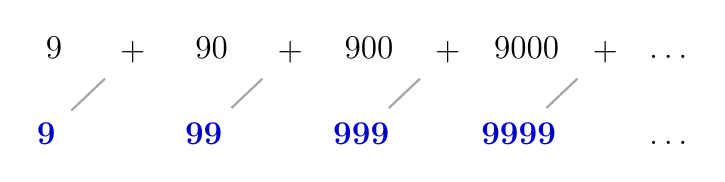
\begin{tikzpicture}[
    term node/.style={font=\large, anchor=base},
    op node/.style={font=\large, anchor=center, yshift=0.5ex},
    sum node/.style={font=\bfseries\large, text=blue!80!black, anchor=base},
    connector line/.style={draw=gray!70, thick, shorten >=3pt, shorten <=3pt}
]

%================CONFIGURATION================
% Set the upper bound for k (e.g., 0 to 5)
% WARNING: Do not set > 8 to avoid "Dimension too large" error
% Partial sums geometric series TikZ
\def\numterms{3} % Limit number of terms to prevent dimension overflow
\def\hunit{1.0} % was 2.0
\def\vsep{1.1} % was 1.8
%=============================================

% Initialize sum
\def\currentSum{0}

\foreach \i [count=\c] in {0,...,\numterms} {

    % --- 1. Calculate Positions ---
    \pgfmathsetmacro{\xTerm}{(\c-1) * 2 * \hunit}
    \pgfmathsetmacro{\xOp}{\xTerm + \hunit}
    \pgfmathsetmacro{\xSum}{\xOp - \vsep}

    % --- 2. Calculate Math ---
    % Calculate 9 * 10^i
    % Use round() to fix floating point precision (e.g. 99.999 -> 100)
    \pgfmathtruncatemacro{\termVal}{round(9 * pow(10, \i))}
    
    % Update sum
    \pgfmathtruncatemacro{\newSum}{\currentSum + \termVal}
    % Global update for the loop
    \global\let\currentSum=\newSum

    % --- 3. Draw Elements ---
    \node[term node] at (\xTerm, \vsep) {\termVal};
    \node[op node] (Op\c) at (\xOp, \vsep) {$+$};
    \node[sum node] (S\c) at (\xSum, 0) {\currentSum};
    \draw[connector line] (S\c) -- (Op\c);

    % --- 4. Handle End Ellipses ---
    % FIX: Check if the current loop iterator (\i) equals the max (\numterms)
    \ifnum\i=\numterms
        \pgfmathsetmacro{\xEllipsis}{\xOp + \hunit*0.8}
        \node[term node] at (\xEllipsis, \vsep) {$\ldots$};
        \node[term node] at (\xEllipsis, 0) {$\ldots$};
    \fi
}

\end{tikzpicture}}
                    \caption{Calculating partial sums for $\displaystyle \sum_{k=0}^n9 \cdot 10^k$.}
                    \label{fig_part_sums_geometric}
                \end{figure}
  
                \begin{table}[hbtp]
                    \centering
                    \begin{tabular}{c|c|c|c|c}
                        $n$ & 1 & 2 & 3 & 4  \\ \hline
                        partial sum  & 9 & 99 & 999 & 9999 \\ \hline 
                        pattern & $10^1-1$ & $10^2-1$ & $10^3-1$ & $10^4-1$ 
                    \end{tabular}
                    \caption{Partial sums for $\displaystyle \sum_{k=0}^n9 \cdot 10^k$.}
                    \label{tab_partial_sums_geometric}
                \end{table}
    
        \end{apart}
\end{exam}

It is your turn to conjecture explicit forms of a sum.

\begin{act}[Sum conjectures]
\label{act_sum_conj}
    For each problem, calculate the first few partial sums and use pattern recognition to complete a conjecture about an explicit formula for the sum.  
        \begin{actpart}
            \item $\displaystyle \sum_{k=0}^n2^k = 1+2+4+\ldots +2^n$
            % Answer = 2^{n+1}-1           
            Hint: The answer involves powers of two.          
            
            \item $\displaystyle \sum_{k=1}^n(2k)=2+4+6+ \ldots + 2n$ % Answer=n(n+1)$          
            Hint: Factor.     
            
            \item \label{part_sum_recip_hs} $\displaystyle \sum_{k=1}^n\frac{2}{k(k+1)}= 1 + \frac{1}{3} + \frac{1}{6} + \ldots+\frac{2}{n(n+1)}$
            
            Use computational technology to find the partial sums as fractions. (In DESMOS, click the fraction icon to ask for the answer as a fraction.)  
            % Answer = 1, 4/3, 3/2, 8/5, 5/3, \ldots = 2/2, 4/3, 6/4, 8/5, 10/6, \ldots = 2n/n+1
        \end{actpart}
\end{act}

Let's look at \Cref{act_sum_conj} (\ref{part_sum_recip_hs}).

\begin{exam}[Explicit form of sum of reciprocals of handshake numbers]
\label{exam_sum_recip_hs_conj}
    Calculate the first few partial sums and use pattern recognition to complete a conjecture about an explicit formula for the sum
        $$\displaystyle \sum_{k=1}^n\frac{2}{k(k+1)}= 1 + \frac{1}{3} + \frac{1}{6} + \ldots+\frac{2}{n(n+1)}.$$
            \begin{soln}  
                The first five partial sums are 
                    $$1, \frac{4}{3}, \frac{3}{2}, \frac{8}{5}, \frac{5}{3}, \frac{12}{7}.$$
                Notice the denominators are of the form     
                    $$\underline{\hspace{.2in}}, 3, \underline{\hspace{.2in}}, 5, \underline{\hspace{.2in}}, 7$$
                which suggests that we should rewrite the fractions over the denominators
                $$2, 3, 4, 5, 6, 7$$
                to get
                    $$\frac{2}{2}, \frac{4}{3}, \frac{6}{4}, \frac{8}{5}, \frac{10}{6}, \frac{12}{7}.$$      
                Next, we make a table showing the index $n$ and the partial sums, as shown in \Cref{tab_partial_sums_recip_hs}.
                Based on this pattern, we conjecture that $$\sum_{k=1}^n\frac{2}{k(k+1)}= \frac{2n}{n+1}.$$
                \end{soln}                    
  
                \begin{table}[hbtp]
                    \centering
                    \begin{tabular}{c|c|c|c|c|c|c}
                        $n$ & 1 & 2 & 3 & 4 & 5 & 6  \\ \hline
                        &&&&&& \\
                        partial sum  & 1 & $\displaystyle \frac{4}{3}$ & $\displaystyle\frac{3}{2}$  & $\displaystyle\frac{8}{5}$ & $\displaystyle\frac{5}{3}$ & $\displaystyle\frac{12}{7}$ \\
                        &&&&&& \\ \hline 
                        &&&&&& \\
                        pattern & $\displaystyle\frac{2}{2}$ & $\displaystyle\frac{4}{3}$ & $\displaystyle\frac{6}{4}$  & $\displaystyle\frac{8}{5}$ & $\displaystyle\frac{10}{6}$ & $\displaystyle\frac{12}{7}$ \\ 
                        &&&&&& 
                    \end{tabular}
                    \caption{Partial sums for $\displaystyle \sum_{k=1}^n\frac{2}{k(k+1)}$.}
                    \label{tab_partial_sums_recip_hs}
                \end{table}
    
\end{exam}

%%%%%%%%%%%%%%%%%%%%%%%%%%%%%%%%%%%%%%%%%%
\newcommand{\subprodconj}{Product Conjectures}
\subsection{\subprodconj}
\label{sub_prod_conj}

Next, we work with products.

\begin{defn}[Partial products]
\label{defn_partial_prod}
   Consider a list of numbers  $a_s, a_{s+1}, a_{s+2}, \ldots, a_n$ for some integers $s$ and $n$. 
        \begin{apart}
            \item For the product  
                $$\prod_{k=s}^n a_k =a_s \times a_{s+1} \times a_{s+2} \times \ldots \times a_n,$$
            the \vocab{partial products} are
                \begin{align*}
                    \prod_{k=s}^s a_k &=a_s,\\
                    \prod_{k=s}^{s+1} a_k &=a_s \times a_{s+1}, \\
                    \prod_{k=s}^{s+2} a_k &=a_s \times a_{s+1} \times a_{s+2},
                \end{align*}
            and so on.  For example, for the product $$\prod_{k=1}^n 2 = 2 \times 2 \times \cdots \times 2,$$ 
            the partial products are
                \begin{align*}
                    \prod_{k=1}^1 2 &=2, \\
                    \prod_{k=1}^2 2 &=2 \times 2=4,\\
                    \prod_{k=1}^3 2 &=2 \times 2 \times 2=8,
                \end{align*}
            and so on.
            \item The \vocab{sequence of partial products} is 
                $$a_s, a_sa_{s+1},a_sa_{s+1}a_{s+2}, \ldots.$$
            For example, the sequence of partial products in our example begins $$2, 4, 8, \ldots.$$
        \end{apart}           
\end{defn}

There is a shorthand notation for calculating partial products that we introduce in our next example, where we revisit the product from \Cref{defn_partial_prod}. 

\begin{exam}[Conjecture explicit form of product of constant.]
\label{exam_partial_prod_conj_constant}
    Consider the product 
        $$\prod_{k=1}^n 2 =2 \times 2 \times 2 \times \ldots \times 2.$$ 
        
        \begin{apart}
            \item Calculate the partial products.
                \begin{soln}
                    We display the partial products using a shorthand in \Cref{fig_part_products_constant}.  
                    At each $\times$ sign, we draw a line and record the product from the beginning to that line.
                \end{soln}
                
                \begin{figure}[hbtp]
                    \centering
                    \scalebox{0.75}{%Used in \Cref{sec_sum_conj}.

% THanks Gemini -- I modified from sum to product myself!

\begin{tikzpicture}[
    % --- Styles ---
    term node/.style={font=\large, anchor=base},
    % Plus node centered for clean line connections
    op node/.style={font=\large, anchor=center, yshift=0.5ex}, 
    % Blue color for products
    prod node/.style={font=\bfseries\large, text=blue!80!black, anchor=base},
    connector line/.style={draw=gray!70, thick, shorten >=3pt, shorten <=3pt}
]

%================CONFIGURATION================
\def\numterms{6}

% Geometry settings
% \hunit: Horizontal spacing
% \vsep: Vertical separation
\def\hunit{1.5} 
\def\vsep{1.8}
%=============================================

% Initialize running product at 1
\def\currentProd{1}

\foreach \i [count=\c] in {1,...,\numterms} {

    % --- 1. Calculate Positions ---
    % Top Term Position
    \pgfmathsetmacro{\xTerm}{(\c-1) * 2 * \hunit}
    
    % Operator Position (x)
    \pgfmathsetmacro{\xOp}{\xTerm + \hunit}
    
    % Bottom Product Position
    % SLOPE 1 CONSTRAINT: xProd = xOp - vsep
    \pgfmathsetmacro{\xProd}{\xOp - \vsep}


    % --- 2. Calculate Math (Product) ---
    \pgfmathsetmacro{\newProd}{int(\currentProd * 2)}
    \global\let\currentProd=\newProd


    % --- 3. Draw Elements ---
    
    % Draw the Number in the Top Row
    \node[term node] at (\xTerm, \vsep) {2};

    % Draw the Plus Sign
    \node[op node] (Op\c) at (\xOp, \vsep) {$\times$};

    % Draw the Partial Product
    \node[prod node] (S\c) at (\xProd, 0) {\currentProd};

    % Draw the Connector Line
    \draw[connector line] (S\c) -- (Op\c);


    % --- 4. Handle End of Sequence (Ellipses) ---
    \ifnum\c=\numterms
        % Calculate positions for ellipses 
        \pgfmathsetmacro{\xTopEllipsis}{\xOp + \hunit*0.8}
        % Maintain vertical alignment with top ellipsis
        \pgfmathsetmacro{\xBottomEllipsis}{\xTopEllipsis} 
        
        \node[term node] at (\xTopEllipsis, \vsep) {$\ldots$};
        % Note: We place the bottom ellipsis directly below the top one
        % to show the sequence continues indefinitely. 
        \node[term node] at (\xTopEllipsis, 0) {$\ldots$};
    \fi
}

\end{tikzpicture}

% \end{document}}
                    \caption{Calculating partial products for $\displaystyle \prod_{k=1}^n2$.}
                    \label{fig_part_products_constant}
                \end{figure}
            \item Display the partial products in a table.
                \begin{soln}
                    We are interested in finding an explicit formula for the product as a function of $n$, so it is helpful to have the partial products in a table, as shown in \Cref{tab_partial_products_constant}.
                \end{soln}
                
                \begin{table}[hbtp]
                    \centering
                    \begin{tabular}{c|c|c|c|c|c|c}
                        $n$ & 1 & 2 & 3 & 4 & 5 & 6 \\ \hline
                        partial product & 2 & 4 & 8 & 16 & 32 & 64 \\ \hline
                        pattern & $2^1$ & $2^2$ & $2^3$ & $2^4$ & $2^5$ & $2^6$
                    \end{tabular}
                    \caption{Partial products for $\displaystyle \prod_{k=1}^n2$.}
                    \label{tab_partial_products_constant}
                \end{table}
            \item Use pattern recognition to conjecture an explicit form.
                \begin{soln}
                    We notice that each partial product is two to the index $n$, and add another row to our table to show the pattern.  We conjecture $\displaystyle \prod_{k=1}^n2=2^n$, which is no surprise since
                    $$ \prod_{k=1}^n2 = \underbrace{2 \times 2 \times \ldots \times 2}_{n \text{ times}}=2^n.$$
                \end{soln}
        \end{apart}
\end{exam}

Observe that we can use each partial product to calculate the next partial product without having to multiply from the beginning.  For example, once we calculate $\displaystyle \prod_{k=1}^32 = 2 \times 2 \times 2 = 8$, we can calculate 
    $$\displaystyle \prod_{k=1}^42 = 2 \times 2 \times 2 \times 2 = (2 \times 2 \times 2)\times 2=8 \times 2=16.$$  
That is, the new partial product is equal to the previous partial product times the new term.
We state this result in general.

\begin{rem}[Recursive definition of partial product]
\label{rem_rec_def_partial_prod}
    Consider a list of numbers $a_s, a_{s+1}, a_{s+2}, \ldots, a_n$ for some integers $s$ and $n$. Then
        \begin{align*}
            \prod_{k=s}^n a_k & = a_s \times a_{s+1} \times \ldots \times a_{n-1} \times a_n \\
            & = (a_s \times a_{s+1}\times \ldots \times a_{n-1}) \times a_n \\
            & = \left(\prod_{k=s}^{n-1} a_k\right) \times  a_n
        \end{align*}
    We can remember this recursion as
        $$\underbrace{\prod_{k=s}^n a_k}_{\text{new product}} 
        = \underbrace{\prod_{k=s}^{n-1} a_k}_{\text{previous product}} 
        \times \underbrace{a_n}_{\text{new term}}$$
\end{rem}

Let's look at another example of calculating partial products and using pattern recognition to conjecture an explicit formula.

\begin{exam}[Conjecture explicit formula for product.]
\label{exam_conj_explicit_prod_linear}
    Calculate the first few partial products, display your findings in a table, and use pattern recognition to conjecture an explicit formula for the product: $\displaystyle \prod_{k=1}^nk$.    
        \begin{soln}
            We start by writing out the first six terms and their partial products, as shown in \Cref{fig_part_product_linear}.  
            For example, $1 \times 2 = 2$.  Next, using the previous product (as in \Cref{rem_rec_def_partial_prod}) we get $1 \times 2 \times 3 = (2) \times 3 = 6$.  Then, $6 \times 4 = 24$, and so on. 
            Next, we make a table showing the index $n$ and the partial products, as shown in \Cref{tab_partial_products_linear}.          
            We recognize these numbers as the factorials (or we realize that we are multiplying consecutive integers).  We show this pattern in the third row of the table.  Based on this pattern, we conjecture that $\displaystyle \prod_{k=1}^nk=n!$, which is no surprise because $1 \times 2 \times 3 \times \cdots \times n = n!$.
                \end{soln}     
                
                \begin{figure}[hbtp]
                    \centering
                    \scalebox{0.75}{\input{Tikz/partial_products_k}}  
                    \caption{Calculating partial products for $\displaystyle \prod_{k=1}^nk$.}
                    \label{fig_part_product_linear}
                \end{figure}
                
                \begin{table}[hbtp]
                    \centering
                    \begin{tabular}{c|c|c|c|c|c|c}
                        $n$ & 1 & 2 & 3 & 4 & 5 & 6 \\ \hline
                        partial product  & 1 & 2 & 6 & 24 & 120 & 720 \\ \hline  
                        pattern & $1!$ & $2!$ & $3!$ & $4!$ & $5!$ & $6!$ 
                    \end{tabular}
                    \caption{Partial products for $\displaystyle \prod_{k=1}^nk$.}
                    \label{tab_partial_products_linear}
                \end{table}
\end{exam}

It is your turn to conjecture explicit forms of a product.

\begin{act}[Product conjectures]
\label{act_prod_conj}
    For each problem, calculate the first few partial products and use pattern recognition to complete a conjecture about an explicit formula for the product.  
        \begin{actpart}
            \item $\displaystyle \prod_{j=1}^n \frac{j+1}{j} = \frac{2}{1} \times \frac{3}{2} \times \frac{4}{3} \times \cdots \times \frac{n+1}{n}$. % Answer: n+1 

            \item $\displaystyle \prod_{k=1}^n(2k) = 2(1) \times 2(2) \times 2(3) \times \cdots \times 2(n)$. 
            Hint: Keep the partial products factored.  Group together the twos to write one factor as a power of two. % 2^nn!
        \end{actpart}
\end{act}

%%%%%%%%%%%%%%%%%%%%%%%%%%%%%%%%%%%%%%%%%%
\newcommand{\subsumfib}{Detour: Fibonacci Sums}
\subsection{\subsumfib}
\label{sub_sum_fib}

There are some interesting identities involving sums of Fibonacci numbers.  Try an example.

\begin{act}[Fibonacci sums conjectures]
\label{act_fib_sums_conj}
    Recall that the Fibonacci numbers are defined by $F_0=0$, $F_1=1$, and $F_n = F_{n-1}+F_{n-2}$ for $n \ge 2$.  The first few Fibonacci numbers are listed in \Cref{tab_15fibs}.

        \begin{table}[hbtp]
            \centering
            \begin{tabular}{ll ll l}
                 $F_0=0$ & $F_1=1$ & $F_2=1$ & $F_3=2$ & $F_4=3$ \\ 
                 $F_5=5$ & $F_6=8$ & $F_7=13$ & $F_8=21$ & $F_9=34$ \\ 
                 $F_{10}=55$ & $F_{11}=89$ & $F_{12} = 144$ & $F_{13} = 233$ & $F_{14} = 377$
            \end{tabular}
            \caption{The first fifteen Fibonacci numbers.}
            \label{tab_15fibs}
        \end{table}

    \begin{apart}
        \item \label{part_fib_sums_even_index} Calculate the first six partial sums and use pattern recognition to conjecture an explicit formula for the sum
            \begin{align*}
                \sum_{k=1}^nF_{2k} & = F_2+F_4+F_6+F_8+F_{10}+F_{12}+\ldots +F_{2n} \\
                & = 1+3+8+21+55+144+ \ldots +F_{2n} 
            \end{align*}
        Hint: Add one to each partial sum to see the pattern.
        
        \item \label{part_Fib_sums_alt_act} Calculate the first six partial sums and use pattern recognition to conjecture an explicit formula for the sum
            \begin{align*}
                \sum_{k=1}^n(-1)^{k+1}F_k & = F_1-F_2+F_3-F_4+F_5-F_6+ \ldots +(-1)^{n+1}F_n \\
                & = 1-1+2-3+5-8+ \ldots +F_{2n} 
            \end{align*}
        Hint: Subtract one from each partial sum to see the pattern.
    \end{apart}
\end{act}

Let's take a closer look at the sum from \Cref{act_fib_sums_conj} (\ref{part_fib_sums_even_index}).

\begin{exam}[Fibonacci sum conjecture]
\label{exam_fib_sum_conj_even_index} 
    Calculate the first six partial sums and use pattern recognition to conjecture an explicit formula for the sum
        \begin{align*}
            \sum_{k=1}^nF_{2k} & = F_2+F_4+F_6+F_8+F_{10}+F_{12}+ \ldots +F_{2n} \\
            & = 1+3+8+21+55+144 \ldots +F_{2n} 
        \end{align*}
    The first fifteen Fibonacci numbers appear in \Cref{tab_15fibs}.
            \begin{soln}
                We start by writing out the first six terms and their partial sums, as shown in \Cref{fig_part_sums_fib}.  For example, $1+3 = 4$.  Next, using the previous sum (as in \Cref{rem_rec_def_partial_sum}) we get $1+3+8 = (4) + 8 = 12$.  Then, $12 + 21 = 33$, and so on. 
                Next, we make a table showing the index $n$ and the partial sums, as shown in \Cref{tab_partial_sums_fib}.        To see the pattern, notice that each partial sum is one less than a Fibonacci number. Notice that the subscripts are odd. We conjecture
                    $$\sum_{k=1}^nF_{2k}=F_{2n+1}-1.$$
                \end{soln}     
                
                \begin{figure}[hbtp]
                    \centering
                    \scalebox{0.75}{\begin{tikzpicture}[
    % --- Styles ---
    term node/.style={font=\large, anchor=base},
    % Plus node centered for clean line connections
    op node/.style={font=\large, anchor=center, yshift=0.5ex}, 
    % Blue color for sums
    sum node/.style={font=\bfseries\large, text=blue!80!black, anchor=base},
    connector line/.style={draw=gray!70, thick, shorten >=3pt, shorten <=3pt}
]

%================CONFIGURATION================
\def\numterms{6}

% Geometry settings
\def\hunit{1.5} 
\def\vsep{1.8}
%=============================================

% Initialize running sum at 0
\def\currentSum{0}

% --- NEW: Initialize Fibonacci Logic ---
% We need F_{2k}. Let's track the current pair (F_{odd}, F_{even}).
% Start with F_1 = 1, F_2 = 1.
\def\fPrev{1} % Represents F_{2k-1} (initially F_1)
\def\fCurr{1} % Represents F_{2k}   (initially F_2)

\foreach \i [count=\c] in {1,...,\numterms} {

    % --- 1. Calculate Positions (Same as before) ---
    \pgfmathsetmacro{\xTerm}{(\c-1) * 2 * \hunit}
    \pgfmathsetmacro{\xOp}{\xTerm + \hunit}
    \pgfmathsetmacro{\xSum}{\xOp - \vsep}


    % --- 2. Calculate Math (Fibonacci Summation) ---
    % Capture the current term (F_2k) for display
    \pgfmathsetmacro{\termValue}{int(\fCurr)}
    
    % Update the Partial Sum
    \pgfmathsetmacro{\newSum}{int(\currentSum + \termValue)}
    \global\let\currentSum=\newSum
    
    % --- 3. Update Fibonacci Numbers for NEXT loop ---
    % We need to jump from (F_{2k-1}, F_{2k}) to (F_{2k+1}, F_{2k+2})
    % Step 1: F_{2k+1} = F_{2k} + F_{2k-1}
    \pgfmathsetmacro{\nextOdd}{int(\fCurr + \fPrev)}
    % Step 2: F_{2k+2} = F_{2k+1} + F_{2k}
    \pgfmathsetmacro{\nextEven}{int(\nextOdd + \fCurr)}
    
    % Global update for the loop
    \global\let\fPrev=\nextOdd
    \global\let\fCurr=\nextEven


    % --- 4. Draw Elements ---
    
    % Draw the Fibonacci Number (F_2k)
    \node[term node] at (\xTerm, \vsep) {$\termValue$};

    % Draw the Plus Sign
    \node[op node] (Op\c) at (\xOp, \vsep) {$+$};

    % Draw the Partial Sum
    \node[sum node] (S\c) at (\xSum, 0) {\currentSum};

    % Draw the Connector Line
    \draw[connector line] (S\c) -- (Op\c);


    % --- 5. Handle End of Sequence (Ellipses) ---
    \ifnum\c=\numterms
        \pgfmathsetmacro{\xTopEllipsis}{\xOp + \hunit*0.8}
        \pgfmathsetmacro{\xBottomEllipsis}{\xTopEllipsis} 
        \node[term node] at (\xTopEllipsis, \vsep) {$\ldots$};
        \node[term node] at (\xTopEllipsis, 0) {$\ldots$};
    \fi
}

\end{tikzpicture}}  
                    \caption{Calculating partial sums for $\displaystyle \sum_{k=1}^nF_{2k}$.}
                    \label{fig_part_sums_fib}
                \end{figure}
                
                \begin{table}[hbtp]
                    \centering
                    \begin{tabular}{c|c|c|c|c|c|c}
                        $n$ & 1 & 2 & 3 & 4 & 5 & 6 \\ \hline
                        partial sum  & 1 & 4 & 12 & 33 & 88 & 232 \\ \hline  
                        pattern & $2-1$ & $5-1$ & $13-1$ & $34-1$ & $89-1$ & $233-1$ \\
                        $=$ & $F_3-1$ & $F_5-1$ & $F_7-1$ & $F_9-1$ & $F_{11}-1$ & $F_{13}-1$\\
                    \end{tabular}
                    \caption{Partial sums for $\displaystyle \sum_{k=1}^nF_{2k}$.}
                    \label{tab_partial_sums_fib}
                \end{table}
\end{exam}

%%%%%%%%%%%%%%%%%%%%%%%%%%%%%%%%%%%%%%%%%%
\newcommand{\subfactorpolys}{Algebra: Factoring Polynomials}
\subsection{\subfactorpolys}
\label{sub_factor_polys}

In some of our conjectures about sums and products, our answer involved a factored polynomial.  We would like to eventually prove these conjectures.  For those proofs, it is helpful to be able to factor polynomials.  As we saw in \Cref{sub_polys}, we use the distributive rule to multiply polynomials.  Let's look at an example using the distributive rule to factor polynomials.

\begin{exam}[Factoring polynomial]
\label{exam_unfoil}  
~
    \begin{apart}
        \item Multiply $(n+s)(n+t)$ and write the answer as a polynomial in the variable $n$.
        \label{part_expand_binomial_general}
            \begin{soln}
                 Using the distributive property (FOIL) as discussed in \Cref{sub_polys}, we get              
                 \begin{center}
                    \begin{tabular}{lll}
                    $(n+s)(n+t)$ &=& $\underbrace{(n)(n)}_{\text{First}} 
                    +\underbrace{(n)(t)}_{\text{Outside}} 
                    + \underbrace{(s)(n)}_{\text{Inside}} + \underbrace{(s)(t)}_{\text{Last}}$ \\ 
                    &=& $n^2 + tn + sn + st$ \\
                    &=& $n^2+ (s+t)n + st$          
                    \end{tabular}
                \end{center}
                Observe that the coefficient $n$ is $s+t$, the sum of $s$ and $t$, and the constant term is $st$, the product of $s$ and $t$.
            \end{soln}
        \item Factor $n^2 -n-6$.
            \begin{soln}
                Based on our observation in (\ref{part_expand_binomial_general}), we might guess that 
                $$n^2 -n-6 = (n+\underline{\quad})(n+\underline{\quad})$$ 
                where the sum of the integers in the blanks is $-1$ and the product of the integers in the blanks is $-6$. We guess that the integers are $-3$ and $2$ and so
                $$\text{answer: }n^2 -n-6 = (n-3)(n+2).$$
                This process of factoring is sometimes nicknamed \vocab{unfoiling}, since we FOIL to check. 
                $$\text{check: }(n-3)(n+2)=n^2 + 2n-3n-6 = n^2-n-6.$$
            \end{soln}
        \item \label{part_diff_sq} Multiply $(n+s)(n-s)$ and write the answer as a polynomial in the variable $n$.
            \begin{soln}
                Multiplying we get
                \begin{center}
                    \begin{tabular}{lll}
                    $(n+s)(n-s)$ &=& $\underbrace{(n)(n)}_{\text{First}} 
                    +\underbrace{(n)(-s)}_{\text{Outside}} 
                    + \underbrace{(s)(n)}_{\text{Inside}} + \underbrace{(s)(-s)}_{\text{Last}}$ \\ 
                    &=& $n^2 - sn + sn - s^2$ \\
                    &=& $n^2-s^2$          
                    \end{tabular}
                \end{center}
            \end{soln}
        \item Factor $n^2 -4$.
            \begin{soln}
                We can use the result of (\ref{part_diff_sq}), $$n^2-4 = n^2-2^2=(n+2)(n-2).$$
            \end{soln}
    \end{apart}
\end{exam}

Practice using the FOIL method to factor polynomials.

\begin{act} [Factoring olynomials]
\label{act_UNFOIL}
~
    \begin{apart}
        \item Factor $m^2+3m+2$.
        \item Factor $m^2-1$.
        \item Factor $2k^2+3k+1$. Hint:  Try a product of the form $(2k + \underline{\quad})(k+\underline{\quad})$. %(2k+1)(k+1)
    \end{apart}
\end{act}

Let's look at another example.

\begin{exam}[Factor quadratic polynomial]
\label{exam_factor_nonmonic_quad}
   Factor $3k^2+2k-1$.  
       \begin{soln}
           Let's try a product of the form $(3k + \underline{\quad})(k+\underline{\quad})$.
           To get the constant term $-1$, one of the blanks must be 1 and the other must be $-1$. Since $$(3k -1)(k+1)=3k^2+3k-k-1=3k^2+2k-1,$$ 
           we can factor $3k^2+2k-1 = (3k -1)(k+1)$.
       \end{soln}
\end{exam}

%%%%%%%%%%%%%%%%%%%%%%%

\subsection{Exercises}

%%%%%%%%%%%%%%%%%%%%%%%%

\subsubsection*{Exercises for \Cref{sub_sum_conj} \subsumconj}

\begin{exer}[\exerP] %  partial sums]
\label{exer_partial_sums}
    Calculate the first five partial sums for each sum.
        \begin{exerpart}
            \item \label{part_partial_sum_powers3} $\displaystyle \sum_{k=0}^n2 \cdot 3^k$
            \item \label{part_partial_sums_constant} $\displaystyle \sum_{i=1}^{n}3$
            \item \label{part_partial_sums_alt} $\displaystyle \sum_{m=0}^{n}(-1)^m$ % alternating
            \item \label{part_partial_sums_square} $\displaystyle \sum_{j=1}^{n}(6j^2)$
        \end{exerpart}  
\end{exer}

\begin{exer}[\exerP] %  sum conjecture]
\label{exer_sum_conj_powers3_constant}
~ 
    \begin{exerpart}
        \item Use the partial sums from \Cref{exer_partial_sums} (\ref{part_partial_sum_powers3}) to conjecture an explicit formula for the sum $\displaystyle \sum_{k=0}^n2 \cdot 3^k$.
          
        \item Use the partial sums from \Cref{exer_partial_sums} (\ref{part_partial_sums_constant}) to conjecture an explicit formula for the sum $\displaystyle \sum_{i=1}^{n}3$.           
    \end{exerpart}
\end{exer}

\begin{exer}[\exerP] %  sum conjecture odds] 
\label{exer_sum_conj_odds}
    Calculate the first few partial sums and use pattern recognition to conjecture an explicit formula for the sum 
        $$\displaystyle \sum_{k=1}^n(2k-1).$$
        % Answer $n^2$  
\end{exer}

\begin{exer}[\exerU] %  sum conjecture alternating or sum of squares]
\label{exer_sum_conj_alt_sum_sq}
~
    \begin{exerpart}
        \item Use the partial sums from \Cref{exer_partial_sums} (\ref{part_partial_sums_alt}) to conjecture an explicit formula for the sum $\displaystyle \sum_{m=0}^{n}(-1)^m$. % alternating
            
        \item Use the partial sums from \Cref{exer_partial_sums} (\ref{part_partial_sums_square}) to conjecture an explicit formula for the sum $\displaystyle \sum_{j=0}^{n}(6j^2)$.  Hint: Factor.
    \end{exerpart}
\end{exer}

\begin{exer}[\exerU] %largest factorial representations]
\label{exer_sum_conj_factorials}
    Calculate the first few partial sums and use pattern recognition to conjecture an explicit formula for the sum
            $$ \sum_{k=1}^nk(k!).$$
    By the way, the result of this exercise is a key step in proving the uniqueness of the factorial representations introduced in \Cref{act_fact_rep}. 
\end{exer}

\begin{exer}[\exerU] %  sum conjecture reciprocal powers of 2]
\label{exer_sum_conj_recip_powers2}
    Calculate the first few partial sums and use pattern recognition to conjecture an explicit formula for the sum 
        $$\displaystyle \sum_{k=0}^n\frac{1}{2^k}.$$    
\end{exer}

\begin{exer}[\exerU] %  sum conjecture new odds] 
\label{exer_sum_conj_new_odds}
    Calculate the first few partial sums and use pattern recognition to conjecture an explicit formula for the sum 
        $$\displaystyle \sum_{k=0}^n(2k+3).$$
        % Answer $n(n+4)$
\end{exer}

\begin{exer}[\exerU] %  sum conjecture powers 5] 
\label{exer_sum_conj_powers5}
    Calculate the first few partial sums and use pattern recognition to conjecture an explicit formula for the sum 
    sum $\displaystyle \sum_{k=1}^n 4 \cdot 5^k$.
        % Answer $5^{n+1}-1$  
\end{exer}

\begin{exer}[\exerU] %  sum conjecture $4k+1$]
\label{exer_sum_conj_4kplus1}
    Calculate the first few partial sums and use pattern recognition to conjecture an explicit formula for the sum 
        $$\displaystyle \sum_{k=0}^n(4k+1).$$
        % $n(2n+1)$$
    
\end{exer}

\begin{exer}[\exerU] %  sum conjecture alternating squares]
\label{exer_sum_conj_alt_sq}
    Calculate the first few partial sums and use pattern recognition to conjecture an explicit formula for the sum 
        $$\sum_{k=1}^n(-1)^kk^2.$$
\end{exer}

\begin{exer}[\exerU] %  sum conjecture $4k-3$]
\label{exer_sum_conj_4kminus3}
    Calculate the first few partial sums and use pattern recognition to conjecture an explicit formula for the sum 
        $$\displaystyle \sum_{k=0}^n(4k-3).$$
        % Answer $n(2n-1)$
    Hint: Factor.   
\end{exer}
 
\begin{exer}[\exerU] %  sum conjecture fraction]
\label{exer_sum_conj_fraction}
    Calculate the first few partial sums and use pattern recognition to conjecture an explicit formula for the sum 
        $$\displaystyle \sum_{k=1}^n\frac{1}{(2k-1)(2k+1)}.$$
        %\frac{1}{3} + \frac{1}{15} + \frac{1}{35} + \ldots+ \frac{1}{(2n-1)(2n+1)} = $   
    Note that DESMOS adds fractions exactly if you click on the fraction icon.
\end{exer}

\begin{exer}[\exerR] % sum conjectures
\label{exer_dyk_sum_conj}
    Do you know \ldots
        \begin{exerpart}
            \item How to calculate a partial sum?
            \item Why it is useful to have a recursive definition of a partial sum?
            \item How to use partial sums and pattern recognition to conjecture an explicit formula for a sum?
        \end{exerpart}
\end{exer}

\begin{exer}[\exerE] %  sum conjecture cubes]
\label{exer_sum_conj_cubes}
    Calculate the first few partial sums and use pattern recognition to conjecture an explicit formula for the sum
    $$\displaystyle \sum_{m=1}^n6m^3.$$
    Hint: Factor.
\end{exer}

\begin{exer}[\exerE] % sum conjecture alternating sum]
\label{exer_sum_conj_alt_sum}
    Calculate the first few partial sums and use pattern recognition to conjecture an explicit formula for the sum $\displaystyle \sum_{k=1}^n(-1)^kk$.  Hint: The formula involves the ceiling.
\end{exer}
%%%% ANSWER $$\displaystyle \sum_{k=1}^n(-1)^kk = (-1)^n\left\lceil\frac{n}{2}\right\rceil $$

%%%%%%%%%%%%%%%%%%%%%%%%

\subsubsection*{Exercises for \Cref{sub_prod_conj} \subprodconj}

\begin{exer}[\exerP] %  partial products]
\label{exer_partial_prod}
    Calculate the first five partial products for each product.
        \begin{exerpart}
            \item \label{part_partial_prod_recip} $\displaystyle \prod_{k=1}^n\frac{1}{k}$
            \item \label{part_partial_prod_3} $\displaystyle  \prod_{i=1}^n3$
            \item \label{part_partial_prod_3k} $\displaystyle \prod_{k=1}^n3k$
            \item \label{part_partial_prod_square} $\displaystyle \prod_{j=1}^nj^2$
        \end{exerpart}    
\end{exer}

\begin{exer}[\exerP] %  product conjecture]
\label{exer_prod_conj_recip_constant}
~
    \begin{exerpart}
        \item Use the partial products from \Cref{exer_partial_prod} (\ref{part_partial_prod_recip}) to conjecture an explicit formula for the product $\displaystyle \prod_{k=1}^n\frac{1}{k}$. % Answer 1/n!
        \item Use the partial products from \Cref{exer_partial_prod} (\ref{part_partial_prod_3}) to conjecture an explicit formula for the product $\displaystyle \prod_{i=1}^n3$ % Answer 3^n
    \end{exerpart}
\end{exer}

\begin{exer}[\exerU] %  product conjectures with factorials]
\label{exer_prod_conj_3k_square}
~
    \begin{exerpart}
        \item Use the partial products from \Cref{exer_partial_prod} (\ref{part_partial_prod_3k}) to conjecture an explicit formula for the product $\displaystyle \prod_{k=1}^n3k$. % Answer 3^nn!
        \item Use the partial products from \Cref{exer_partial_prod} (\ref{part_partial_prod_square}) to conjecture an explicit formula for the product $\displaystyle \prod_{j=1}^nj^2$. % Answer (n!)^2
    \end{exerpart}
\end{exer}

\begin{exer}[\exerU] %  product conjecture $1 - \frac{1}{j}$]
\label{exer_prod_conj_1minus1overj}
    Calculate the first few partial products and use pattern recognition to conjecture an explicit formula for the product 
        $$\displaystyle \prod_{j=2}^n \left(1 - \frac{1}{j}\right).$$ %n 
\end{exer} 

\begin{exer}[\exerU] %  product conjecture twice a square]
\label{exer_prod_conj_twice_sq}
    Calculate the first few partial products and use pattern recognition to conjecture an explicit formula for the product   
        $\displaystyle  \prod_{j=1}^n(2j^2).$
\end{exer}

\begin{exer}[\exerU] %  product conjecture $\frac{2}{j}$]
\label{exer_prod_conj_2overj}
    Calculate the first few partial products and use pattern recognition to conjecture an explicit formula for the product  
        $\displaystyle \prod_{j=1}^n \frac{2}{j}.$ % Answer 2^n/n!   
\end{exer}

\begin{exer}[\exerR] % product conjectures
\label{exer_dyk_product_conj}
    Do you know \ldots
        \begin{exerpart}
            \item How to calculate a partial product?
            \item Why it is useful to have a recursive definition of a partial product?
            \item How to use partial products and pattern recognition to conjecture an explicit formula for a product? 
        \end{exerpart}
\end{exer}

%%%%%%%%%%%%%%%%%%%%%%%%

\subsubsection*{Exercises for \Cref{sub_sum_fib} \subsumfib}

\begin{exer} [\exerP] %  sum first $n$ Fibonaccis conjecture] 
\label{exer_sum_firstn_Fib_conj}
    Calculate the first six partial sums and conjecture an explicit form for the sum
        \begin{align*}
            \sum_{k=1}^nF_k
            & = F_1+F_2+F_3+F_4+F_5+ + \ldots +F_n \\
            & =1 + 1 + 2 + 3 + 5 +\ldots + F_n.
        \end{align*}
     % Answer $F_{n+2}-1$
\end{exer}

\begin{exer}[\exerU] % sum first $n$ Fibonaccis squared conjecture]
\label{exer_sum_firstn_Fib_sq_conj}
    Calculate the first six partial sums and conjecture an explicit form for the sum
            \begin{align*}
                \sum_{k=1}^n(F_k)^2
                & = F_1^2+F_2^2+F_3^2+F_4^2+F_5^2+\ldots+F_n^2 \\
                & = 1^2+1^2+2^2+3^2+5^2+\ldots + F_n^2.
            \end{align*}  
    % Answer $F_nF_{n+1}$
\end{exer}

\begin{exer}[\exerU] % Sum of odd term Fibs
\label{exer_fib_sum_odd_terms_conj} 
    Calculate the first six partial sums and conjecture an explicit form for the sum
            \begin{align*}
                \sum_{k=1}^{n}F_{2k-1}
                & = F_1+F_3 +F_5 +F_7+F_9+ \ldots + F_{2n-1} \\
                & = 1+2+5+13+34+\ldots + F_{2n-1}.
            \end{align*}
            %Answer: $1, 3, 8, 21, 55, 144, \ldots = F_{2n}$
\end{exer}

\begin{exer}[\exerR] % fibonacci sums
\label{exer_dyk_fib_sums}
    Do you know \ldots
        \begin{exerpart}
            \item How to calculate a partial sum that involves Fibonacci numbers?
            \item How to use partial sums and pattern recognition to conjecture an explicit formula for a sum involving Fibonacci numbers? 
        \end{exerpart}
\end{exer}

%%%%%%%%%%%%%%%%%%%%%%%%

\subsubsection*{Exercises for \Cref{sub_factor_polys} \subfactorpolys}
% %%%%%%%%%%%%%%%%%%
% \subsubsection{\answers for \Cref{sub_factor_polys} \subfactorpolys}

\begin{exer}[\exerP] %  factoring quadratic polynomials]
\label{exer_factor_quad_poly}
~
    \begin{exerpart}
        \item Factor $n^2-n-2$
        \item Factor $n^2+5n+4$.
        \item Factor $n^2+5n-6$.
        \item Factor $n^2-9$.
    \end{exerpart}
\end{exer}

\begin{exer}[\exerU] %  Simplify and factor]
\label{exer_simplify_factor}
    Expand each expression, simplify, then factor the answer as much as possible.
        \begin{exerpart}
            \item $(n-1)n + 2n$
            \item $n(2n-1)+(4n+1)$
            \item $(n-1)n(2n-1) + 6n^2$
        \end{exerpart}
\end{exer}

\begin{exer}[\exerR] % factoring polynomials
\label{exer_dyk_factor_polys}
    Do you know \ldots
        \begin{exerpart}
            \item What is means to factor a polynomial?
            \item How to factor a quadratic polynomial?
            \item How to factor the difference of squares? 
        \end{exerpart}
\end{exer}
%%%%%%%%%%%%%%%%%%%%%%%%%%%
\subsection{\answers}
%%%%%%%%%%%%%%%%%%%%%%%%%%%

%%%%%%%%%%%%%%%%%%
\subsubsection{\answers for \Cref{sub_sum_conj} \subsumconj}

\subsubsection*{\Cref{exer_partial_sums} \answers}
\begin{apart}
    \item Hint: $2, 8, 26, \ldots$
    \item Hint: $3, 6, 9, \ldots$
    \item Hint: $1, 0, 1, \ldots$
    \item Hint: $6, 30, 84, \ldots$
\end{apart}

\subsubsection*{\Cref{exer_sum_conj_powers3_constant} \answers}
\begin{apart}
    \item Hint: The answer involves a power of three, but not exactly $3^n$
    \item Hint: The answer is a multiple of 3.
\end{apart}

\subsubsection*{\Cref{exer_sum_conj_odds} \answers}
Hint: The partial sums are $1, 4, 9, \ldots$.

\subsubsection*{\Cref{exer_sum_conj_alt_sum_sq} \answers}
\begin{apart}
    \item Hint: Use $(-1)^n$ to get a closed formula, noting that $\frac{1}{2} + \frac{1}{2} =1$ and $\frac{1}{2} - \frac{1}{2} =0$.
    \item Hint: $6 = (1)(2)(3)$ and $30 = (2)(3)(5)$.  The first factor equals $n$, what are the next two factors, in terms of $n$?
\end{apart}

\subsubsection*{\Cref{exer_sum_conj_factorials} \answers}
Hint: The partial sums begin $1, 5, 23, \ldots$ and the formula involves factorials, but not exactly $n!$.

\subsubsection*{\Cref{exer_sum_conj_recip_powers2} \answers}
 Hint: The partial sums are $1, \frac{3}{2}, \frac{7}{4}, \ldots$. One version of the formula is a fraction in which the numerator involves a power of two (but not exactly $2^n$) and the denominator is $2^n$.  

\subsubsection*{\Cref{exer_sum_conj_new_odds} \answers}
Hint: Factor the partial sums.

\subsubsection*{\Cref{exer_sum_conj_powers5} \answers}
Hint: The formula involves powers of five, but not exactly $5^n$.

\subsubsection*{\Cref{exer_sum_conj_4kplus1} \answers}
 Hint: Factor the partial sums.

%%%%%%%%%%%%%%%%%%
\subsubsection{\answers for \Cref{sub_prod_conj} \subprodconj}

\subsubsection*{\Cref{exer_partial_prod} \answers}
\begin{apart}
    \item Hint: $\displaystyle 1, \frac{1}{2}, \frac{1}{6}, \ldots$.
    \item Hint: $3, 9, 27, \ldots$.
    \item Hint: $3, 18, 162, \ldots$.
    \item Hint: $1, 4, 36, \ldots$.
\end{apart}

\subsubsection*{\Cref{exer_prod_conj_recip_constant} \answers}
\begin{apart}
    \item Hint: The answer involves factorial.
    \item Hint: The answer involves a power of three.
\end{apart}

\subsubsection*{\Cref{exer_prod_conj_3k_square} \answers}
\begin{apart}
    \item Hint: Keep the partial products factored: $(3 \cdot 1), (3 \cdot 1)(3 \cdot 2),(3 \cdot 1)(3 \cdot 2)(3 \cdot 3), $  Then collect the threes.
    \item Hint: Keep the partial products factored: $(1 \cdot 1),(1 \cdot 1)(2 \cdot 2), (1 \cdot 1)(2 \cdot 2)(3 \cdot 3) $. The answer involves factorials.
\end{apart}

\subsubsection*{\Cref{exer_prod_conj_1minus1overj} \answers}
Hint: $1 - \frac{1}{2} = \frac{1}{2}$, $1 - \frac{1}{3} = \frac{2}{3}$, $1 - \frac{1}{4} = \frac{3}{4}$, so our product is $ \frac{1}{2}\cdot \frac{2}{3} \cdot \frac{3}{4} \cdots $ and, therefore, the partial product are $\frac{1}{2}, \frac{1}{3}, \frac{1}{4}, \ldots$.

\subsubsection*{\Cref{exer_prod_conj_twice_sq} \answers}
Hint: Keep the partial products factored: $(2\cdot 1 \cdot 1),(2\cdot 1 \cdot 1)(2\cdot 2 \cdot 2),(2\cdot 1 \cdot 1)(2\cdot 2 \cdot 2)(2\cdot 3 \cdot 3) , \ldots$.  Then collect twos.

\subsubsection*{\Cref{exer_prod_conj_2overj} \answers}
Hint: Keep the numerator and denominator factored and do not reduce the fractions.

%%%%%%%%%%%%%%%%%%
\subsubsection{\answers for \Cref{sub_sum_fib} \subsumfib}

\subsubsection*{\Cref{exer_sum_firstn_Fib_conj} \answers}
Hint: The formula involves Fibonacci numbers.  For example, $12 = 13-1 = F_7-1$.

\subsubsection*{\Cref{exer_sum_firstn_Fib_sq_conj} \answers}
Hint: The formula involves Fibonacci numbers. Another hint: Factor.

\subsubsection*{\Cref{exer_fib_sum_odd_terms_conj} \answers}
Hint: the answers involved Fibonacci numbers. For example, $55 = F_{10}$.






